\subsubsection{Working with matrixes}\label{workingwithmatrixes}
To facilitate the explanation from this point, we proceed to explain different parts of the network and their mathematical notation with some simplification.
\newline

The following definition of a neural network is used as a starting point:


\begin{figure}[H]
    \centering
    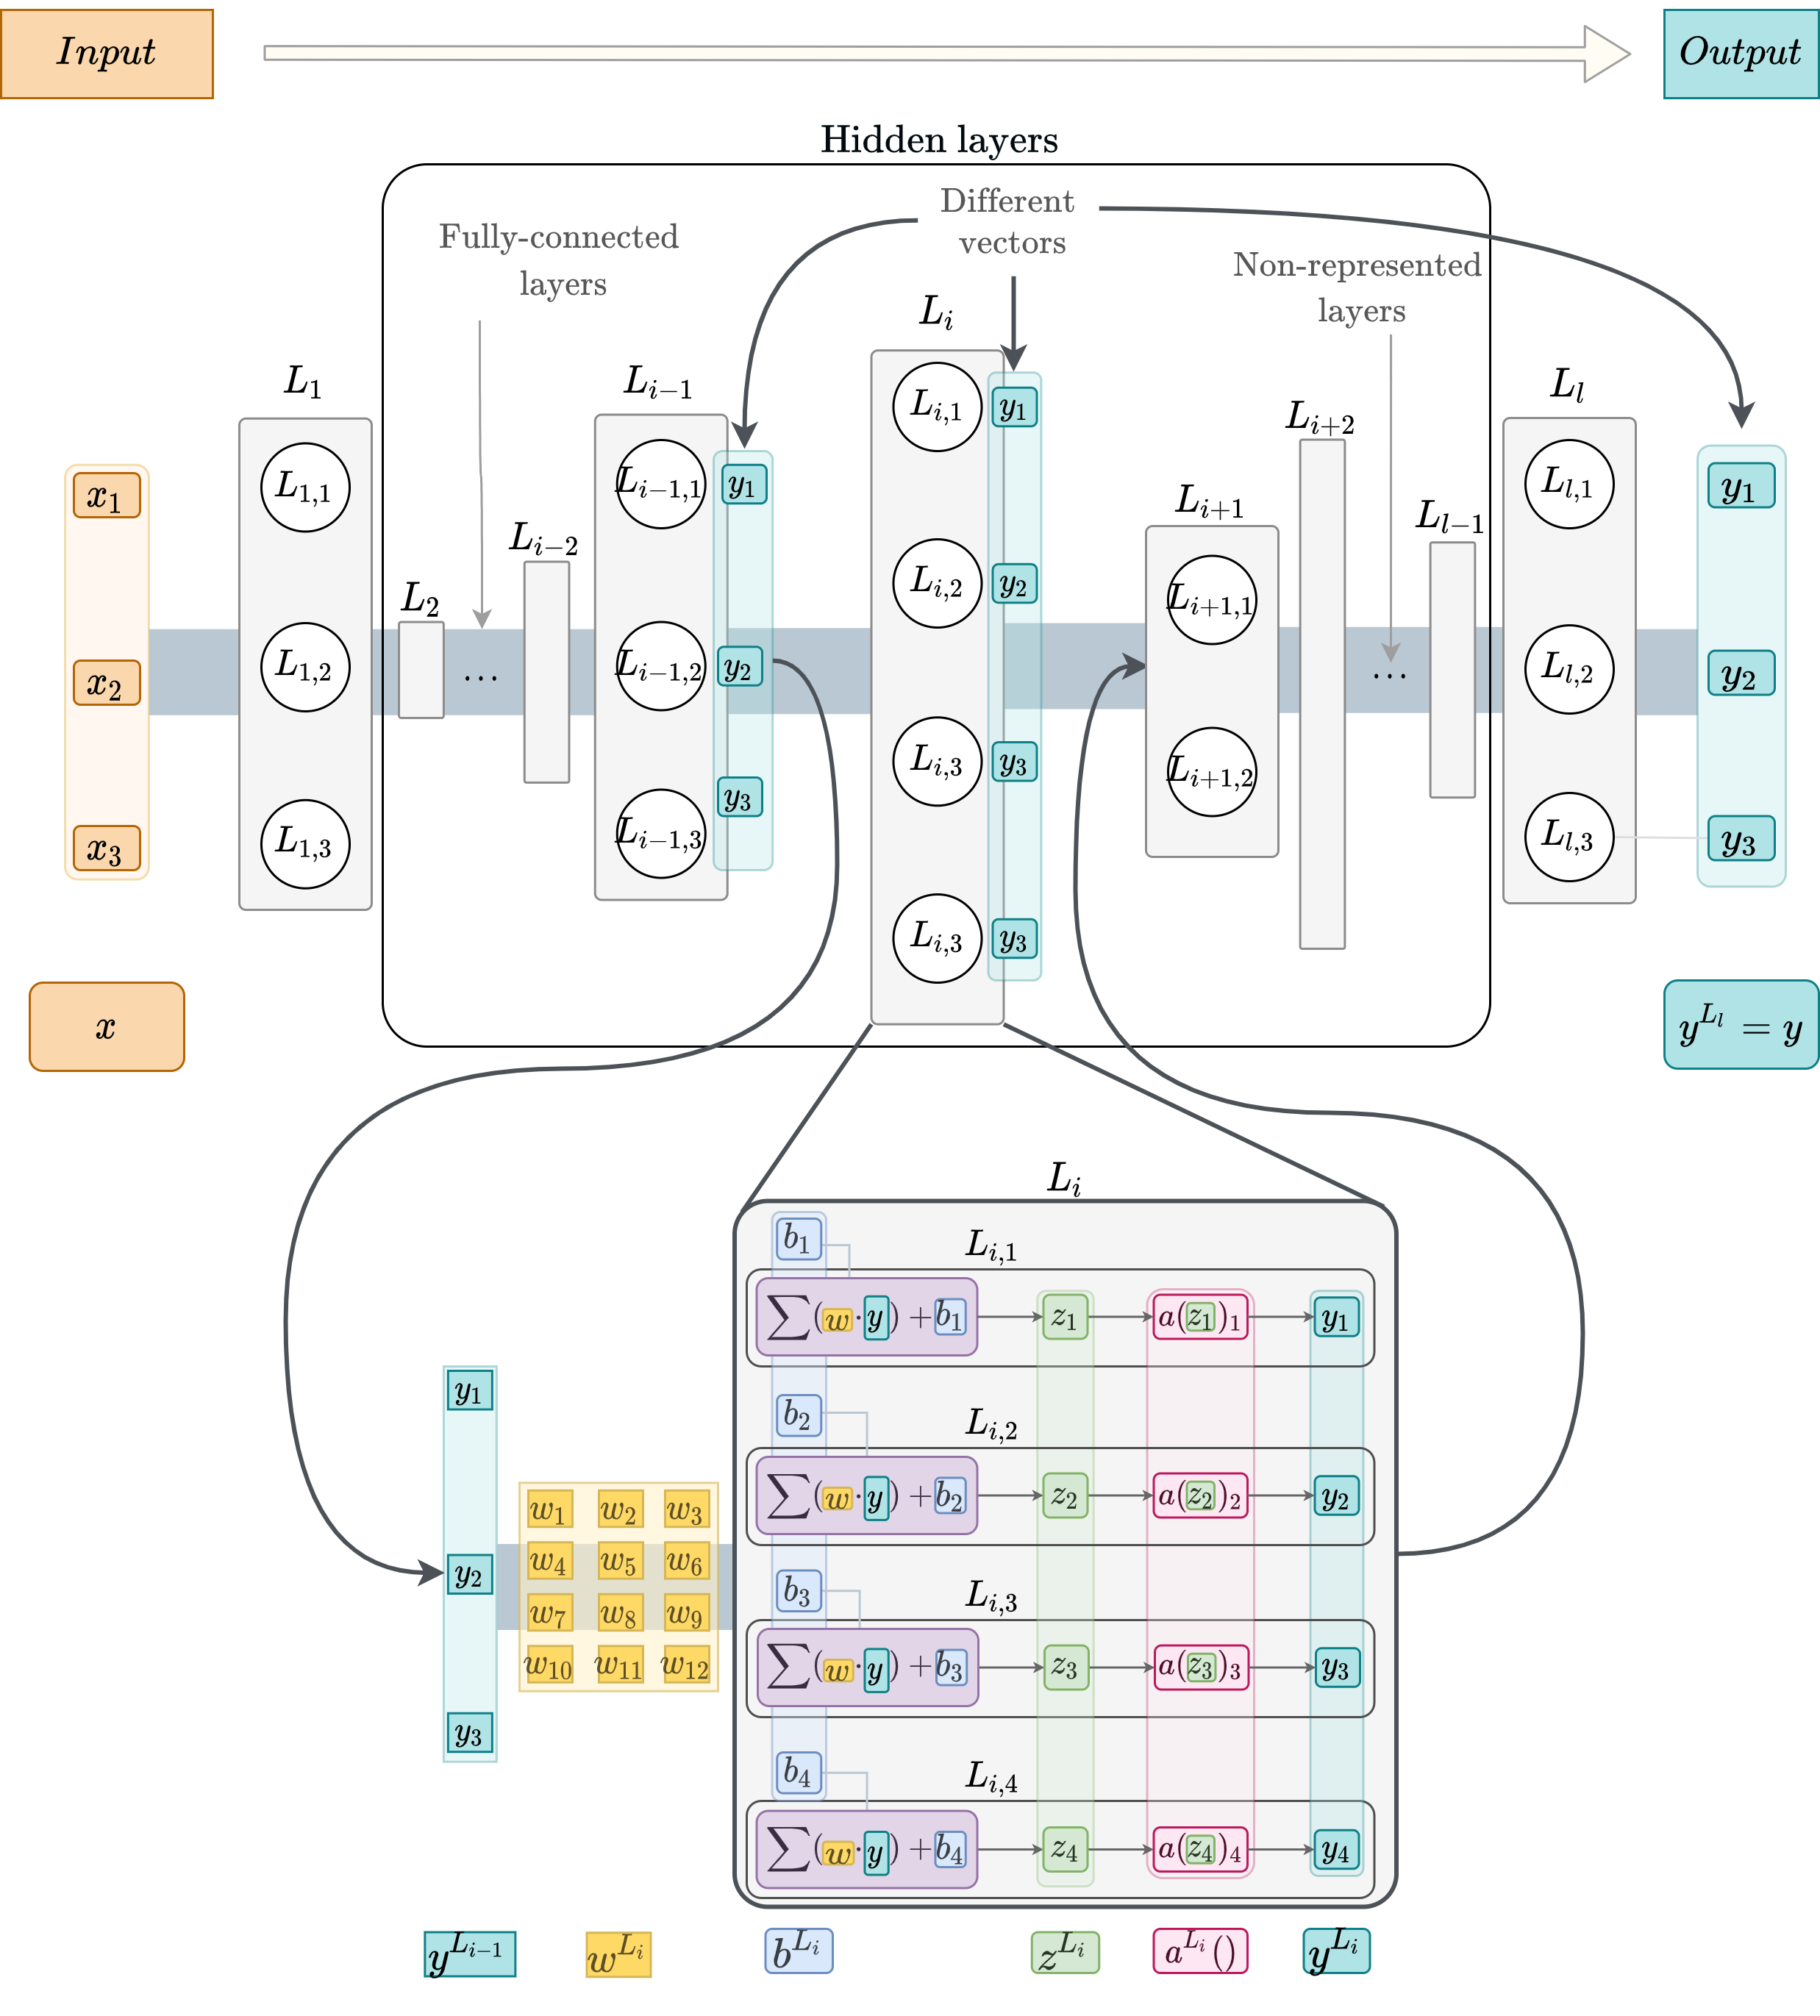
\includegraphics[width=16cm]{images/state-of-art/matrixes/layer_activation_representation.png}
    \caption{Forward pass in \acrshort{nn}.}
    \label{fig:basic_network51}
\end{figure}

The network represented needs three input values that return a single value, so the model will be trained so that, given a vector of three elements, the model will calculate three other elements. The value returned by the model will be equal to the value $y$, calculated in the last layer:

\begin{equation}
    \begin{split}
    y = a^{L_l}(z_l) &= w_l \cdot a^{L_{l-1}}(z_{l-1}) + b_l \\ 
    \text{where}~L_l &= \text{Last layer} \\
  ~w_^{L_l} &= \text{Weights in last layer} \\ 
  ~b_l &= \text{Biases in last layer } \\
  ~a^{L_{u}}(z_{u}) &= \text{Result of the activation function of the} L_{u} \text{layer on the vector } z_u\\
  ~a^{L_{l-1}}(z_{l-1}) &= \text{Vector with the values of the penultimate layer output}
  \end{split}
  \label{eqn:layer3}
\end{equation}


The number of $z_{l-1}$ elements will be the same number of neurons as there are in the $L__{l-1}$ layer. This occurs $\forall z_i$. The $z_{l-1}$ vector is calculated in the $L_{l-1}$ layer as follows:
\begin{equation}
    z_{L_{l-1}} = w_{L_{l-1}} \cdot a^{L_{l-2}}(z_{L_{l-2}}) + b_{L_{l-1}}
  \label{eqn:layer2}
\end{equation}


This process will be repeated until the $z_1$ is calculated:
\begin{equation}
    \begin{split}
    z_1 &= w_1 \cdot x + b_1 \\
    \text{where}~x &= \text{Input vector}
  \end{split}
  \label{eqn:layer1}
\end{equation}

To refer to a layer of the network, $L_i$ will be used, where $i$ is the index of the layer ($i=1$ for the first layer, $i=2$ for the second layer...). To refer to the last layer, $L_l$ will be used, the penultimate one will be $L_{l-1}$ and so on. A second index can be added to refer to a neuron such that $L_{i,j}$ and like the layer index, if $j=1$, will refer to the first neuron in the layer, if $j=2$, will refer to the second neuron in the layer and so on respectively. As an example, the third neuron in the second layer will be referred to as $L_{2, 3}$.
\newline


The vector $w$ and the value $b$ of $L_{2, 3}$ will be referenced such that $w^{L_{2,3}}$ and $b^{L_{2,3}}$ respectively. If we want to refer to a specific value of vector w we will use a third index such as $w^{L_{i,j}}_k$. For example, it will refer to the first weight of the third neuron in the second layer.
\newline


Knowing this new notation, the equations will be simplified from this point on. Therefore, the parameters of a neuron will come in a single vector by adding the value $b$ to the already existing vector $w$. All the vectors will be grouped forming a matrix $W$, where each row will be the vector associated with a neuron. That is, the parameters of a layer $L_i$ will be given as a matrix which will be referred to as $W$.


\begin{equation}
\centering
    \begin{split}
    W^{L_i} &= \begin{pmatrix}
  b^{L_{i,1}} & w^{L_{i, 1}}_1 & w^{L_{i, 1}}_2 & \cdots & w^{L_{i, 1}}_n \\
  b^{L_{i,2}} & w^{L_{i, 2}}_1 & w^{L_{i, 2}}_2 & \cdots & w^{L_{i, 2}}_n \\
  b^{L_{i,3}} & w^{L_{i, 3}}_1 & w^{L_{i, 3}}_2 & \cdots & w^{L_{i, 3}}_n \\
  \vdots & \vdots  & \vdots & & \vdots \\
  b^{L_{i,m}} & w^{L_{i, m}}_1 & w^{L_{i, m}}_2 & \cdots & w^{L_{i, m}}_n
  \end{pmatrix} \\ 
    \text{where}~i &= \text{Index of the layer in the network} \\
  ~n &= \text{Number of neurons in} L_{i-1}\text{ or input vector length if } i=1 \\
  ~m &= \text{Number of neurons in the } L_i \text{ layer}
  \end{split}
  \label{examplenn51}
\end{equation}

As an example, the $W^{L-1}$ matrix of a neural network with 4 neurons in the second last layer and 3 neurons in the third last layer is:

\begin{equation}
  W^{L_{l-1}} = W^{L_2} = \begin{pmatrix}
  b_1 & w_1 & w_2 & w_3 \\
  b_2 & w_4 & w_5 & w_6 \\ 
  b_3 & w_7 & w_8 & w_9 \\ 
  b_4 & w_{10} & w_{11} & w_{12}
  \end{pmatrix} 
  \label{eqn:matrixlayer}
\end{equation}


Using the example in figure \ref{fig:xorgatenetwork}, where specific values are used for $w$ and $b$, the matrices of each layer with the parameters would be such that:

\begin{equation}
  W^{L_1} = \begin{pmatrix}
  0 & 1 & 1 \\ 
  -1 & 1 & 1
  \end{pmatrix}
\end{equation}

\begin{equation}
  W^{L_2} = \begin{pmatrix}
  -2 & 3 & -2
  \end{pmatrix}
\end{equation}


With this new notation in a single matrix, the parameters that need to be calculated in the regression are collected. In fact, this matrix is what the model will have to "learn" in order to get better results. This will be discussed in more detail in section \ref{training}.
\newline


In equation \ref{eqn:activationfunctionbasic} the value was calculated with the function $a()$ of the neuron. From this point, an activation function will receive a vector with the $z$ values of each neuron and therefore this function $a()$ will also return a vector of the same size. In the first layer of a network, this vector will be calculated in such a way that:

\begin{equation}
  y_1 = a^{L_1}(z) = a(W^{L_1}x)
  \label{eqn:activationmatrixwrong}
\end{equation}


But by defining the $W$-matrix in this way, the $W^{L_1}x$ product is impossible to calculate. This can be demonstrated using the example in the equation \ref{examplenn51}. The dimension of $W^{L_1}$ is $(3 \times 6)$. However, the $x$-vector with which it is going to be multiplied has a dimension $(1 \times 5)$. To solve this problem, a $1$ will be added to vector $x$, a vector known as $x'$, and the transposition of this vector will be performed. In this way it will be possible to multiply the matrix $W$ with dimension $3\times6$ with a vector of dimension $6\times1$.

\begin{equation}
\centering
    \begin{split}
  a^L_1(z) &= a(W^{L_2}x') \\
    \text{where}~x' &= [[1] \oplus x]^T = [1, x_1, x_2, ... x_n]^T \\
    n &= \text{Vector size } x \\
    A \oplus B &: \text{Concatenation of vectors } A \text{ and } B
  \end{split}
  \label{eqn:newactivationsimple}
\end{equation}

The rest of the layers do not have this problem. The vector obtained in the previous layer already fulfils the necessary conditions to be able to produce a matrix by a vector. The vector $a^{L_2}(z)$ will use the same equation as equation \ref{eqn:activationmatrixwrong}, but the variable $x$ will be the vector $y$ calculated in the previous layer:

\begin{equation}
  a^{L_2}(z) = a(W^{L_2} \cdot a(W^{L_1}x'))
\end{equation}

This process will be carried out until the last layer of the network is reached. More information can be found in section \ref{feedforward}.
\newline

Also updating equations  \ref{eqn:layer3}, \ref{eqn:layer2} and \ref{eqn:layer1}:

\begin{equation}
    y = a^{L_3}(z_3) = W^{L_3} \cdot a^{L_2}(z_2) 
\end{equation}
\begin{equation}
    z_2 = W^{L_2} \cdot a^{L_1}(z_1)
\end{equation}
\begin{equation}
    z_1 = W^{L_1} \cdot x'
\end{equation}

Grouping all the equations into one, the value of $y$ in a neural network of three layers is given by:
\begin{equation}
    y = a(W^{L_3} \cdot (a(W^{L_2} \cdot (a(W^{L_1} \cdot x')^{L_1}))^{L_2}))^{L_3}
    \label{eqn:feedforwardexample}
\end{equation}

This equation is the one that solves the model in order to obtain the $y$-value and is what is known as the forward-pass algorithm.
\newline